% %%%%%%%%%%%%%%%%%%%%%%%%%%%%%%%%%%%%%%%%%%%%%%%%%%%%%%%%%%%%%%%%%%%%%%%
%   This document is a heavily modified version of the 
%	NIST Technical report developed by K. Miller, kmm5@nist.gov 
%%%%%%%%%%%%%%%%%%%%%%%%%%%%%%%%%%%%%%%%%%%%%%%%%%%%%%%%%%%%%%%%%%%
\documentclass[12pt, twoside]{article}
\usepackage{amsmath}
\usepackage{amsfonts}   % if you want the fonts
\usepackage{amssymb}    % if you want extra symbols
\usepackage{graphicx}   % need for figures
\usepackage{xcolor}
\usepackage{bm}
\usepackage{secdot}		
\usepackage{mathptmx}
\usepackage{float}
\usepackage[utf8]{inputenc}
\usepackage{textcomp}
\usepackage[hang,flushmargin,bottom]{footmisc} % footnote format
\usepackage{fancyhdr}
\usepackage[useregional]{datetime2}
\usepackage{blindtext}
\pagestyle{fancy}

\usepackage{titlesec}
\titleformat{\section}{\normalsize\bfseries}{\thesection.}{1em}{}	% required for heading numbering style
\titleformat*{\subsection}{\normalsize\bfseries}

\usepackage{tocloft}	% change typeset, titles, and format list of appendices/figures/tables
\renewcommand{\cftdot}{}	
\renewcommand{\contentsname}{Table of Contents}
\renewcommand{\cftpartleader}{\cftdotfill{\cftdotsep}} % for parts
\renewcommand{\cftsecleader}{\cftdotfill{\cftdotsep}}
\renewcommand\cftbeforesecskip{\setlength{4pt}{}}
\addtolength{\cftfignumwidth}{1em}
\renewcommand{\cftfigpresnum}{\figurename\ }
\addtolength{\cfttabnumwidth}{1em}
\renewcommand{\cfttabpresnum}{\tablename\ }
\setlength{\cfttabindent}{0in}    %% adjust as you like
\setlength{\cftfigindent}{0in} 

\usepackage{enumitem}         % to control spacing between bullets/numbered lists

\usepackage[numbers,sort&compress]{natbib} % format bibliography 
\renewcommand{\bibsection}{}
\setlength{\bibsep}{0.0pt}

\usepackage{hyperref}
\hypersetup{
	colorlinks = true,
	urlcolor = {blue},
	% linkbordercolor = {blue}
	% urlbordercolor = {blue}
	% citebordercolor = {blue}
	% pdfborderstyle = {/S/U/W 1}
	citecolor = {.},
	linkcolor = {blue},
	anchorcolor = {.},
	filecolor = {.},
	menucolor = {.},
	runcolor = {.}
	pdftitle={},
	pdfsubject={},
	pdfauthor={},
	pdfkeywords={}
}
\urlstyle{same}

\usepackage{epstopdf} % converting EPS figure files to PDF

\usepackage{fancyhdr, lastpage}	% formatting document, calculating number of pages, formatting headers
\setlength{\topmargin}{-0.5in}
\setlength{\headheight}{35pt}
\setlength{\oddsidemargin}{0.25in}
\setlength{\evensidemargin}{0.25in}
\setlength{\textwidth}{6.0in}
\setlength{\textheight}{8.5in}

\usepackage{caption} % required for Figure labels
\captionsetup{font=small,labelfont=bf,figurename=Fig.,labelsep=period,justification=raggedright} 

\pdfminorversion=7

%%%%%%%%%%%%%%%%%%%%%%%%%%%%%%%%%%%%%%%%%%%%%%%%%%%%%%%%%%%%%%%%%%%
%%%%%%%%%%%%%%%%%%%%%%%%%%%%%%%%%%%%%%%%%%%%%%%%%%%%%%%%%%%%%%%%%%%
%%%%%%%%%%%%%%%%%%%%%%%%%%%%%%%%%%%%%%%%%%%%%%%%%%%%%%%%%%%%%%%%%%%
\setcounter{secnumdepth}{3}
\newcommand{\versionnumber}{0.1.9}

%%%%%%%%%%%%%%%%%%%%%%%%%%%%%%%%%%%%%%%%%%%%%%%%%%%%%%%%%%%%%%%%%%%
%	Document
%%%%%%%%%%%%%%%%%%%%%%%%%%%%%%%%%%%%%%%%%%%%%%%%%%%%%%%%%%%%%%%%%%%

\begin{document}
\urlstyle{rm} % Format style of \url   

%%%%%%%%%%%%%%%%%%%%%%%%%%%%%%%%%%%%%%%%%%%%%%%%%%%%%%%%%%%%%%%%%%%%
%	Title 
%%%%%%%%%%%%%%%%%%%%%%%%%%%%%%%%%%%%%%%%%%%%%%%%%%%%%%%%%%%%%%%%%%%%
\begin{titlepage}
\begin{figure}
\begin{tabular}{@{}l@{}}

\includegraphics[width=25cm]{mne-cpp_logo_notext.png}
\end{tabular}
\end{figure}


\begin{flushright}
\vspace{12pt}  
\vfill
\LARGE{\textbf{MNE-CPP Project}} \\

\Huge{\textbf{User and Developer Documentation}} \\
\Huge{\textbf{Version \versionnumber}} \\
% \vfill
\vspace{20pt}
\LARGE{Date: \today} \\
\vfill
% \large Lorenz Esch \\
% \large Gabriel Motta \\
% \large Juan Garcia-Prieto \\
% \vspace{12pt}
% \textit{Athinoula A. Martinos Center for Biomedical Imaging}\\
% \textit{Department of Radiology, Massachusetts General Hospital}\\
% \textit{Harvard Medical School}\\
% \textit{Boston, MA}
% \vspace{12pt}
% \vfill


\end{flushright}
\end{titlepage}
\let\cleardoublepage\clearpage


%%%%%%%%%%%%%%%%%%%%%%%%%%%%%%%%%%%%%%%%%%%%%%%%%%%%%%%%%%%%%%%%%%%%
%   Disclamer - Information page
%%%%%%%%%%%%%%%%%%%%%%%%%%%%%%%%%%%%%%%%%%%%%%%%%%%%%%%%%%%%%%%%%%%%

\begin{titlepage}
\noindent \normalsize This document has been generated automatically. \\
It is a printable version of the \href{https://mne-cpp.github.io}{MNE-CPP Project documentation web page}\footnote{https://mne-cpp.github.io}.
\vfill
\noindent\normalsize \textbf{MNE Toolbox and the applications contained in the project are available free of charge.} \\
\vfill	
\noindent
\footnotesize \noindent \textbf{Terms of Use: Certain commercial entities, equipment, or materials may be identified in this document in order to describe an experimental procedure or concept adequately. Such identification is not intended to imply recommendation or endorsement by the National Institute of Standards and Technology, nor is it intended to imply that the entities, materials, or equipment are necessarily the best available for the purpose.}\\ 
\vfill
\footnotesize License terms...
\vfill
\end{titlepage}


%%%%%%%%%%%%%%%%%%%%%%%%%%%%%%%%%%%%%%%%%%%%%%%%%%%%%%%%%%%%%%%%%%%%
%   Inspirational Quote
%%%%%%%%%%%%%%%%%%%%%%%%%%%%%%%%%%%%%%%%%%%%%%%%%%%%%%%%%%%%%%%%%%%%
\begin{titlepage}
\begin{flushright}
\vspace*{\fill}
\noindent\normalsize\textbf{If the tools are good, nature will give a clear answer to a clear question.} \\
\textit{Dyson F (1999) The Sun, the Genome, the Internet. \\Oxford University Press, New York} \\
\vspace*{\fill}
\end{flushright}
\end{titlepage}

%%%%%%%%%%%%%%%%%%%%%%%%%%%%%%%%%%%%%%%%%%%%%%%%%%%%%%%%%%%%%%%%%%%%

\fancyhf{}
\fancyhead[LE]{
\includegraphics[width=4cm]{mne-cpp_logo.png}}
\fancyhead[CE]{Version: \versionnumber}
\fancyhead[RE]{\today}
\fancyhead[LO]{\nouppercase\leftmark}
\fancyhead[RO]{\nouppercase\rightmark}
\renewcommand{\subsectionmark}[1]{\markright{\thesubsection\ #1}}
\setlength\headheight{26pt}
\fancyheadoffset{0cm} 

\fancyfoot[LE,RO]{\thepage}

% \section*{Foreword}
% \pagenumbering{roman}
% \normalsize Delete if not applicable\\
% \section*{Preface}
% \normalsize Delete if not applicable\\
% \section*{Abstract}
% \normalsize Required\\
% \section*{Key words}
% \normalsize Required, alphabetized, separated by semicolon, and end in a period.\\
% \pagebreak

%%%%%%%%%%%%%%%%%%%%%%%%%%%%%%%%%%%%%%%%%%%%%%%%%%%%%%%%%%%%%%%%%%%%
%   Table of Contents - Glossary
%%%%%%%%%%%%%%%%%%%%%%%%%%%%%%%%%%%%%%%%%%%%%%%%%%%%%%%%%%%%%%%%%%%%

{
  \hypersetup{linkcolor=black}
  \tableofcontents
  \vfill
  \pagebreak
  % \listoftables
  % \pagebreak
  % \listoffigures
  % \pagebreak
  \section*{Glossary}
  \pagebreak
}


%%%%%%%%%%%%%%%%%%%%%%%%%%%%%%%%%%%%%%%%%%%%%%%%%%%%%%%%%%%%%%%%%%%%
%   Start body of text - page number starts with "1"
%%%%%%%%%%%%%%%%%%%%%%%%%%%%%%%%%%%%%%%%%%%%%%%%%%%%%%%%%%%%%%%%%%%%
\part{HOME}
\label{sec:intro}
MNE-CPP is a cross-platform, open-source framework which offers a variety of software tools to the neuroscientific research community. We provide applications for the acquisition and processing of MEG/EEG data, both in real-time and offline. All applications are built on top of our cross-platform library which is available via an API and can be used to develop new tools.
\blindtext[2]
\section{SectionA}\label{sec:SectionA}
\blindtext[3]
This can be seen in Eq. (1) and Table 1 \cite{Roberts1982}. Information about flowers is available in Sec.~\ref{sec:intro}.\footnote{NIST disclaimer text here.}

% \begin{equation}
% {x}^{n} + {y}^{n} = {z}^{n}
% \end{equation}
%%%%%%%%%%%%%%%%%%%%%%%%%%%%%%%%%%%%%%%%%%%%%%%%%%%%%%%%%%%%%%%%%%%%
%   Equation references are “Eq. (X)��.
% 	“Equation (1) is used at beginning of sentence.
%	Equations are numbered (#) on the right, per the standard LaTeX format
%%%%%%%%%%%%%%%%%%%%%%%%%%%%%%%%%%%%%%%%%%%%%%%%%%%%%%%%%%%%%%%%%%%%
\subsection{SubsectionAX}\label{ssec:subsectionAX}
\blindtext[5]
\subsection{SubsectionAY}\label{ssec:subsectionAY}
\blindtext[2]
\subsubsection{SubsubsectionY}\label{ssec:subsubsectionY}
\blindtext[2]


\begin{table}[H]
	\centering
	\caption{Title.}
	\small
	\begin{tabular}{cc}
		\hline
		ColumnA & ColumnB \\ \hline
		text & text{\scriptsize $^{\rm a}$} \\
		text & text \\
		text & text \\
		text & text \\
		\hline
	\end{tabular}
	
	{\footnotesize 	{\scriptsize $^{\rm a}$}Footnote}
\end{table}

\section{Section2}\label{ssec:section2}
\blindtext[2]
\subsection{Section2SubsectionX}\label{ssec:section2subsectionx}
\subsubsection{SubsubsectionZ}\label{ssec:subsubsectionZ}
\blindtext[3]

%%%%%%%%%%%%%%%%%%%%%%%%%%%%%%%%%%%%%%%%%%%%%%%%%%%%%%%%%%%%%%%%%%%%
%   Tables should appear after they are mentioned in the text. 
%	Superscripted letters (a, b, c, etc.) should be used for table footnotes.
%%%%%%%%%%%%%%%%%%%%%%%%%%%%%%%%%%%%%%%%%%%%%%%%%%%%%%%%%%%%%%%%%%%%
\begin{figure}[h] 
	\centering 	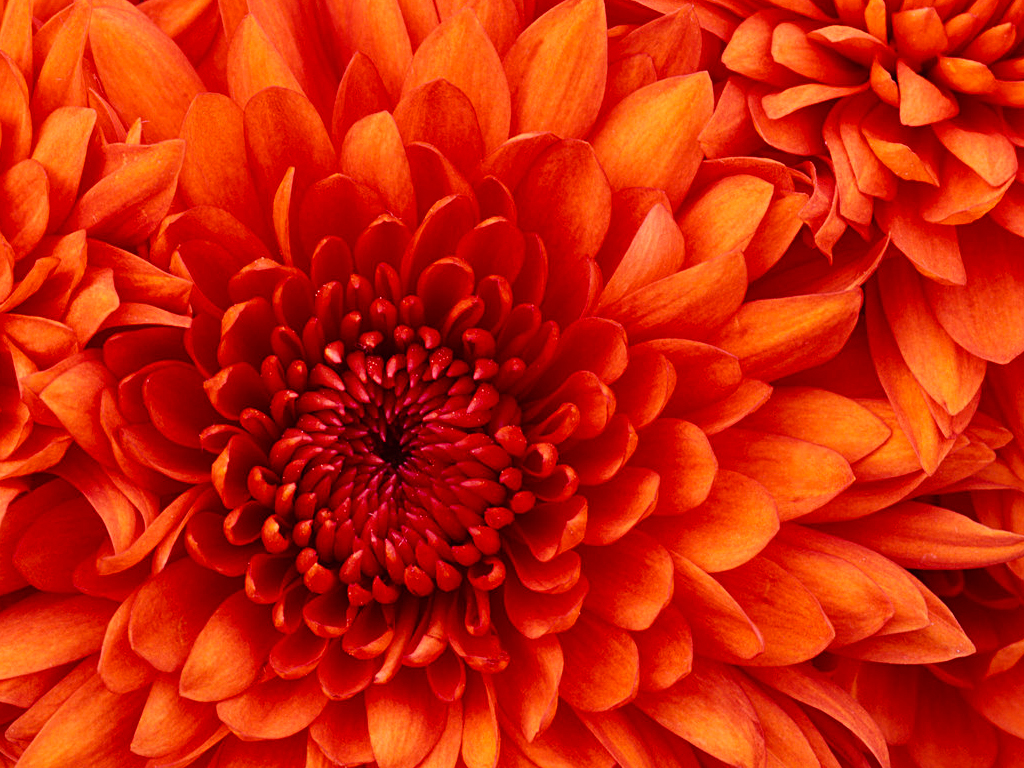
\includegraphics[width=0.5\linewidth]{Chrysanthemum.jpg}
	\caption{This is the caption text.}
	\label{fig:Chrysanthemum}
\end{figure}
%%%%%%%%%%%%%%%%%%%%%%%%%%%%%%%%%%%%%%%%%%%%%%%%%%%%%%%%%%%%%%%%%%%%
%   Figure references are “Fig. X��.
% 	“Figure X�� is used at beginning of sentence. 
% 	Figures should appear after they are mentioned in the text.
%	Figures must have embedded alternate text or “alt text�� in order 
%	to comply with Section 508 accessibility standards. 
%%%%%%%%%%%%%%%%%%%%%%%%%%%%%%%%%%%%%%%%%%%%%%%%%%%%%%%%%%%%%%%%%%%%
\subsubsection{SubsubsectionX}\label{ssec:subsubsectionX2}
\blindtext[2]


\part{References}
% \addcontentsline{toc}{section}{References}
\bibliographystyle{techpubs}
\bibliography{References}

%%%%%%%%%%%%%%%%%%%%%%%%%%%%%%%%%%%%%%%%%%%%%%%%%%%%%%%%%%%%%%%%%%%%
%   Please use the techpubs BibTeX style when compiling bibliography, or follow the instructions on tinyurl.com/techpubsnist to format your .bib / .bbl file appropriately.
%%%%%%%%%%%%%%%%%%%%%%%%%%%%%%%%%%%%%%%%%%%%%%%%%%%%%%%%%%%%%%%%%%%%

% \section*{Appendix A: Supplemental Materials}
% \addcontentsline{toc}{section}{Appendix A: Supplemental Materials}
% Brief description of supplemental files\\

% \section*{Appendix B: Change Log}
% \addcontentsline{toc}{section}{Appendix B: Change Log}
% If updating document with errata, detail changes made to document – delete if not applicable. \\

\end{document}
